% !TEX root = ../proyect.tex

\chapter{Análisis de requisitos}\label{cap:requisitos}

Este capítulo recoge el análisis de requisitos del sistema Linceus Assistant en su versión correspondiente al cierre del prototipo (fase 1). El análisis ha sido un proceso iterativo: la propuesta inicial planteaba un alcance amplio que incluía notificaciones a estudiantes, soporte multilingüe e integraciones en tiempo real con plataformas institucionales, pero la limitación de tiempo propia de un trabajo individual ha obligado a priorizar el núcleo conversacional y el dominio académico, y a aplazar el resto a iteraciones posteriores. La sección~\ref{sec:req-evolucion} cierra el capítulo precisamente con un repaso de cómo ha evolucionado el alcance respecto del documento original, dado que la guía de referencia~\cite{segura2024guiatfg} recomienda dejar trazabilidad de las desviaciones de planificación.

Los requisitos se organizan en cuatro tipos siguiendo la práctica habitual en ingeniería del software: requisitos funcionales (qué hace el sistema), requisitos de información (qué datos maneja), requisitos no funcionales (con qué calidad lo hace) y prototipos de interfaz (cómo se muestra al usuario). Cada requisito funcional se acompaña, cuando procede, de los identificadores de los casos de prueba que lo verifican, lo que permite cruzarlo con el Capítulo~\ref{cap:pruebas}.

\section{Identificación de actores}\label{sec:req-actores}

El sistema atiende a tres tipos de usuarios bien diferenciados, que justifican la estructura de los manuales recogida en el Capítulo~\ref{cap:manuales}.

El \textbf{estudiante} es el usuario principal del prototipo. Comprende tanto al alumnado matriculado en la ETSII como al alumnado de nuevo ingreso o internacional que utiliza el sistema antes de iniciar el curso. Interactúa con el bot a través del \textit{widget} integrado en la página principal, sin necesidad de autenticación, y formula consultas en español natural sobre asignaturas, horarios y profesorado.

El \textbf{administrador del sistema} es el perfil técnico encargado de mantener actualizada la base de conocimiento. Su interacción se realiza exclusivamente a través del panel de administración (puerto 5050), e incluye la sincronización de centros, titulaciones y asignaturas desde Sevius, la vectorización de planes docentes en el módulo RAG y la auditoría de las conversaciones registradas durante el piloto. La existencia del panel obedece principalmente a un requisito de \textbf{mantenibilidad y escalabilidad}: el sistema debe poder ser asumido por otra persona tras el cierre del TFG sin necesidad de manipular directamente la base de datos.

El \textbf{desarrollador} es el perfil destinado a continuar el proyecto en futuras iteraciones. Consume el repositorio, las convenciones documentadas y los registros de decisiones técnicas para incorporar nuevas intenciones, ampliar el dominio o modificar las acciones existentes. Sus requisitos se materializan en buenas prácticas y trazabilidad, no en funcionalidades específicas del producto.

\section{Requisitos funcionales}\label{sec:req-funcionales}

Los requisitos funcionales se agrupan por dominio. La columna \textit{Pruebas} de cada tabla indica los identificadores de los casos de aceptación que verifican el requisito en el Capítulo~\ref{cap:pruebas}.

\subsection{Dominio de asignaturas}\label{subsec:rf-asignaturas}

\begin{table}[hbtp]
\centering
\small
\caption{Requisitos funcionales del dominio de asignaturas.}\label{tab:rf-asignaturas}
\begin{tabular}{|p{1.1cm}|p{8.2cm}|p{1.0cm}|p{2.0cm}|}
\hline
\textbf{ID} & \textbf{Descripción} & \textbf{Prio.} & \textbf{Pruebas} \\ \hline
RF-A1 & El sistema debe responder con la ficha completa de una asignatura cuando el usuario la nombra de forma explícita o mediante alias o acrónimo (ADDA, FP, IISSI2). & Alta & E-P01..E-P12 \\ \hline
RF-A2 & El sistema debe devolver listados de asignaturas filtrados por curso, cuatrimestre, tipo (formación básica, obligatoria, optativa) o créditos. & Alta & L-P01..L-P10 \\ \hline
RF-A3 & El sistema debe responder al conteo de asignaturas que cumplan un criterio dado. & Media & C-P01..C-T02 \\ \hline
RF-A4 & El sistema debe recuperar información del plan docente (criterios de evaluación, profesorado, bloques, idioma, tribunales) mediante el módulo RAG. & Alta & §\ref{subsec:rag-profundidad} \\ \hline
RF-A5 & El sistema debe heredar el contexto cuando una consulta elíptica (``y cuántos créditos tiene?'') se refiere a la última asignatura mencionada. & Media & E-S01..E-S03 \\ \hline
RF-A6 & El sistema debe resolver consultas multi-asignatura en un único turno (``cómo se evalúan DP1 y PSG2''). & Media & E-M01 \\ \hline
RF-A7 & El sistema debe distinguir entre la pregunta ``qué es X'' (ficha) y ``cuándo es X'' (horario), aun cuando ambas comparten léxico. & Alta & E-P09, HA-P01 \\ \hline
\end{tabular}
\end{table}

\subsection{Dominio de horarios}\label{subsec:rf-horarios}

\begin{table}[hbtp]
\centering
\small
\caption{Requisitos funcionales del dominio de horarios.}\label{tab:rf-horarios}
\begin{tabular}{|p{1.1cm}|p{8.2cm}|p{1.0cm}|p{2.0cm}|}
\hline
\textbf{ID} & \textbf{Descripción} & \textbf{Prio.} & \textbf{Pruebas} \\ \hline
RF-H1 & El sistema debe devolver el horario semanal de un curso y grupo dados. & Alta & H-P01..H-P11 \\ \hline
RF-H2 & El sistema debe devolver el horario filtrado por día de la semana. & Alta & H-P01, H-P10 \\ \hline
RF-H3 & El sistema debe filtrar el horario por cuatrimestre cuando el usuario lo especifica. & Media & H-PC01..H-PC03 \\ \hline
RF-H4 & El sistema debe responder al horario de una asignatura concreta sin requerir curso ni grupo. & Alta & HA-P01..HA-P12 \\ \hline
RF-H5 & El sistema debe distinguir aulas de teoría de aulas de laboratorio cuando el usuario lo solicita expresamente. & Media & HA-P11 \\ \hline
RF-H6 & El sistema debe solicitar curso y grupo cuando la consulta los requiere y faltan en el mensaje. & Alta & H-P10, H-P12 \\ \hline
RF-H7 & El sistema debe rechazar de manera explícita consultas con curso o grupo inexistentes (curso 8, grupo 15). & Media & H-N01, H-N02 \\ \hline
\end{tabular}
\end{table}

\subsection{Dominio de profesorado}\label{subsec:rf-profesorado}

\begin{table}[hbtp]
\centering
\small
\caption{Requisitos funcionales del dominio de profesorado.}\label{tab:rf-profesorado}
\begin{tabular}{|p{1.1cm}|p{8.2cm}|p{1.0cm}|p{2.0cm}|}
\hline
\textbf{ID} & \textbf{Descripción} & \textbf{Prio.} & \textbf{Pruebas} \\ \hline
RF-P1 & El sistema debe devolver los datos de contacto de un profesor (email, despacho, teléfono, web personal) por nombre o apellido. & Alta & P-P01..P-P10 \\ \hline
RF-P2 & El sistema debe listar el profesorado que imparte una asignatura. & Alta & P-PA01..P-PA08 \\ \hline
RF-P3 & El sistema debe identificar al coordinador y a los suplentes de una asignatura mediante recuperación semántica sobre el plan docente. & Alta & P-PA05..P-PA08 \\ \hline
RF-P4 & El sistema debe responder a consultas sobre tutorías redirigiendo al correo del profesor (decisión de diseño documentada en D-061). & Media & P-T01..P-T05 \\ \hline
RF-P5 & El sistema debe permitir filtrar el profesorado de un departamento concreto. & Media & P-P10 \\ \hline
RF-P6 & El sistema debe tolerar errores tipográficos moderados en nombres de profesores (``parejjo'', ``galinndo''). & Media & P-W01..P-W07 \\ \hline
RF-P7 & El sistema debe declarar explícitamente la ausencia de información cuando un profesor no figura en la base de datos, sin inventar contenido. & Alta & P-N01..P-N04 \\ \hline
\end{tabular}
\end{table}

\subsection{Comportamientos transversales}\label{subsec:rf-transversal}

\begin{table}[hbtp]
\centering
\small
\caption{Requisitos funcionales transversales.}\label{tab:rf-transversal}
\begin{tabular}{|p{1.1cm}|p{8.2cm}|p{1.0cm}|p{2.0cm}|}
\hline
\textbf{ID} & \textbf{Descripción} & \textbf{Prio.} & \textbf{Pruebas} \\ \hline
RF-T1 & El sistema debe permitir cambiar dinámicamente la titulación activa durante una conversación, ya sea desde el selector o mediante lenguaje natural. & Alta & CC-P01..CC-P11 \\ \hline
RF-T2 & El sistema debe rechazar titulaciones fuera del alcance ETSII con un mensaje explícito (\textit{cambia a Biología}). & Alta & CC-N01 \\ \hline
RF-T3 & El sistema debe identificar consultas fuera de ámbito (clima, peticiones generales) y responder de forma cortés sin entrar al pipeline de consulta académica. & Alta & F-01..F-04 \\ \hline
RF-T4 & El sistema debe bloquear intentos de \textit{prompt injection} y \textit{jailbreak} (``ignora las instrucciones anteriores''). & Alta & R-01..R-04 \\ \hline
RF-T5 & El sistema debe ofrecer un mensaje de bienvenida y soportar la pregunta meta-conversacional ``¿qué eres?'' redirigiendo a la naturaleza del bot. & Media & R-04 \\ \hline
RF-T6 & El sistema debe permitir al usuario reportar respuestas incorrectas mediante un mecanismo de \textit{feedback} integrado en el \textit{widget}. & Media & --- \\ \hline
\end{tabular}
\end{table}

\subsection{Funcionalidades del panel de administración}\label{subsec:rf-admin}

El panel de administración no se ofrece al estudiante final, sino al perfil de administrador descrito en la Sección~\ref{sec:req-actores}. Su existencia responde a un requisito de mantenibilidad: garantizar que la persona que asuma la continuidad del sistema pueda gestionar los datos sin necesidad de manipular directamente la base de datos. Los requisitos se recogen en la Tabla~\ref{tab:rf-admin}.

\begin{table}[hbtp]
\centering
\small
\caption{Requisitos funcionales del panel de administración.}\label{tab:rf-admin}
\begin{tabular}{|p{1.1cm}|p{8.2cm}|p{1.0cm}|}
\hline
\textbf{ID} & \textbf{Descripción} & \textbf{Prio.} \\ \hline
RF-AD1 & El panel debe permitir la navegación jerárquica Centro $\rightarrow$ Titulación $\rightarrow$ Asignatura sobre los datos cargados (D-037). & Alta \\ \hline
RF-AD2 & El panel debe ofrecer la sincronización de centros, titulaciones y asignaturas desde Sevius como fuente de verdad institucional, mediante un flujo \textit{preview-first} (D-038, D-039). & Alta \\ \hline
RF-AD3 & El panel debe permitir vectorizar el plan docente de una asignatura, integrándolo en el corpus de \textit{embeddings} consumido por el módulo RAG (D-040, D-041). & Alta \\ \hline
RF-AD4 & El panel debe importar y enriquecer profesorado a partir del directorio PDI de \texttt{us.es} usando el filtro de centro (D-043, D-044). & Media \\ \hline
RF-AD5 & El panel debe ofrecer una vista jerárquica Centro $\rightarrow$ Departamento $\rightarrow$ Profesor, con un \textit{bucket} para profesores sin departamento asignado (D-051). & Media \\ \hline
RF-AD6 & El panel debe exponer las conversaciones registradas en \texttt{conversation\_log} para revisión manual del evaluador, con la posibilidad de marcarlas como revisadas. & Alta \\ \hline
RF-AD7 & El panel debe agregar el \textit{feedback} explícito por turno aportado por los usuarios y permitir su consulta agregada. & Media \\ \hline
\end{tabular}
\end{table}

\section{Requisitos de información}\label{sec:req-informacion}

El modelo de información del sistema se estructura en torno a tres bloques. El primero recoge los datos de \textbf{dominio académico} consumidos por el bot, que son la fuente de verdad para responder a las consultas del usuario. El segundo recoge los datos del \textbf{módulo RAG}, esto es, los fragmentos vectorizados de los planes docentes con sus respectivos \textit{embeddings}. El tercero recoge los datos de \textbf{operación}, es decir, las conversaciones registradas durante el piloto y el \textit{feedback} explícito asociado.

\subsection{Entidades de dominio}\label{subsec:ri-dominio}

Las entidades del dominio académico son las recogidas en la Tabla~\ref{tab:ri-dominio}. La descripción técnica completa de cada tabla, con sus tipos, claves y restricciones, figura en el Capítulo~\ref{cap:estructura-bd}.

\begin{table}[hbtp]
\centering
\small
\caption{Entidades de información del dominio académico.}\label{tab:ri-dominio}
\begin{tabular}{|p{2.8cm}|p{9.0cm}|}
\hline
\textbf{Entidad} & \textbf{Descripción} \\ \hline
Centro & Unidad organizativa que agrupa titulaciones (ETSII). \\ \hline
Titulación & Plan de estudios (GII-IS, GII-IC, GII-TI). \\ \hline
Asignatura & Materia con su código, créditos, curso, cuatrimestre y tipo. \\ \hline
Departamento & Unidad académica responsable del profesorado. \\ \hline
Profesor & Docente con datos de contacto, despacho y departamento. \\ \hline
Profesor-Asignatura & Relación que vincula un profesor con la docencia de una asignatura, con el grupo y el rol (titular, coordinador, suplente). \\ \hline
Grupo de clase & Asignatura impartida en un grupo concreto a un curso. \\ \hline
Aula & Espacio físico identificado por código (A0.10, B1.31, F1.30) y tipo (teoría/laboratorio). \\ \hline
Horario & Sesión docente que vincula grupo, aula, día, franja horaria y cuatrimestre. \\ \hline
Plan docente & Documento PDF oficial asociado a una asignatura, fuente del corpus RAG. \\ \hline
\end{tabular}
\end{table}

\subsection{Entidades del módulo RAG}\label{subsec:ri-rag}

El módulo RAG opera sobre fragmentos textuales (\textit{chunks}) extraídos de los planes docentes. Cada \textit{chunk} se almacena junto con su \textit{embedding} vectorial calculado con el modelo de \textit{embeddings} de Gemini, y con un conjunto de metadatos que permiten filtrar y reordenar resultados durante la recuperación: titulación, asignatura, sección del plan docente (profesorado, evaluación, bloques, etc.), grupo y curso. La sección como metadato fue una decisión de diseño documentada (D-031, D-058.b): se usa como señal para reordenar resultados pero no como filtro estricto, dado que la sección de origen no siempre es informativa para responder a la pregunta.

\subsection{Entidades de operación}\label{subsec:ri-operacion}

La operación del sistema en producción registra dos entidades. La tabla \texttt{conversation\_log} almacena turno a turno cada interacción con el bot: identificador anónimo de sesión, mensaje del usuario, \textit{intent} clasificado, \textit{slots} activos, respuesta del bot, indicador de revisión manual y marca temporal. La tabla \texttt{feedback} recoge la valoración explícita del usuario sobre un turno concreto cuando este utiliza los botones de aprobación o rechazo del \textit{widget}. Ninguna de las dos almacena datos personales identificables, dado que la sesión es anónima por diseño.

\section{Requisitos no funcionales}\label{sec:req-no-funcionales}

Los requisitos no funcionales se enuncian en términos medibles y se cruzan con la evidencia recogida en el Capítulo~\ref{cap:pruebas}. Los umbrales son los que el equipo del TFG considera aceptables para un prototipo de fase 1 desplegable a la población de la ETSII; se han ajustado durante el desarrollo a la luz de las cifras observadas durante el piloto.

\begin{table}[hbtp]
\centering
\small
\caption{Requisitos no funcionales y evidencia.}\label{tab:rnf}
\begin{tabular}{|p{1.4cm}|p{4.5cm}|p{4.0cm}|p{2.5cm}|}
\hline
\textbf{ID} & \textbf{Descripción} & \textbf{Umbral} & \textbf{Evidencia} \\ \hline
RNF-1 & Latencia mediana de respuesta extremo a extremo. & p50 $\leq$ 4~s & §\ref{subsec:no-funcional-latencia} (3,4~s) \\ \hline
RNF-2 & Latencia en cola larga. & p95 $\leq$ 12~s & §\ref{subsec:no-funcional-latencia} (10,5~s) \\ \hline
RNF-3 & Coste medio por turno (servicio Gemini). & $\leq$ 0,05 cts & §\ref{subsec:no-funcional-coste} (0,012~cts) \\ \hline
RNF-4 & Tasa de éxito en suite de aceptación E2E. & $\geq$ 90~\% & §\ref{sec:pruebas-e2e} (94,3~\%) \\ \hline
RNF-5 & Tasa de éxito sobre tráfico real post-despliegue. & $\geq$ 85~\% & §\ref{sec:pruebas-trafico} (98,3~\%) \\ \hline
RNF-6 & Disponibilidad del servicio. & $\geq$ 99~\% mensual & Pendiente fase 2 \\ \hline
RNF-7 & Idioma soportado. & Español peninsular & Validado en piloto \\ \hline
RNF-8 & Compatibilidad de navegadores. & Chrome, Firefox, Edge y Safari modernos. & Verificado manualmente \\ \hline
RNF-9 & Diseño \textit{responsive} en dispositivos móviles. & Funcional en pantallas $\geq$ 320~px. & Verificado manualmente \\ \hline
RNF-10 & Anonimato del usuario y ausencia de PII. & Sesiones identificadas mediante UUID anónimo. & Por diseño \\ \hline
RNF-11 & Reproducibilidad del despliegue. & \textit{Stack} levantable mediante \texttt{docker compose up}. & §\ref{sec:manual-despliegue} \\ \hline
RNF-12 & Trazabilidad de decisiones técnicas. & Registro en \texttt{docs/sprints/}. & Sprints S2--S7 \\ \hline
\end{tabular}
\end{table}

Conviene comentar dos requisitos en particular. El cumplimiento de la \textbf{normativa de protección de datos} (RNF-10) se materializa por construcción más que por restricciones de despliegue: el sistema no requiere autenticación, no almacena datos personales identificables, y los datos académicos consultados (planes docentes, horarios, directorio de profesorado) son de carácter público y proceden de fuentes oficiales (Sevius, \texttt{us.es}). La propuesta inicial contemplaba un despliegue \textit{on-premise} como mecanismo de garantía adicional; en la implementación final, dado que la información tratada no incluye datos sensibles, se ha optado por un despliegue en infraestructura externa (DigitalOcean y Supabase) que simplifica la operación sin comprometer la privacidad del usuario.

El requisito de \textbf{soporte multilingüe}, que figuraba como funcional en la propuesta original, se ha reformulado y aplazado: el corpus académico está mayoritariamente redactado en español, los modelos de \textit{embeddings} y de generación se han ajustado al castellano y la dotación de tiempo del prototipo no permitía abrir un segundo flujo de pruebas para el inglés. La sección~\ref{sec:req-evolucion} lo recoge entre las funcionalidades aplazadas a fase 2.

\section{Prototipos de interfaz}\label{sec:req-prototipos}

El prototipo no se ha apoyado en herramientas de \textit{wireframing} (Figma o similares) durante la fase de diseño: la interfaz se ha construido directamente sobre código HTML/CSS/JS \textit{vanilla}, tomando como referencia la identidad visual de \texttt{www.us.es} (decisión D-027) para garantizar coherencia con el ecosistema institucional. La validación visual y de usabilidad se ha realizado de forma iterativa contra los \textit{stakeholders} del piloto, incorporando los cambios identificados durante el feedback (D-029, D-030).

A continuación se recogen las capturas de las dos interfaces principales. Su inserción definitiva queda como tarea de redacción final de la memoria.

\begin{figure}[hbtp]
\centering

\includegraphics[width=0.95\linewidth]{img/conversacion_ejemplo.png}
\caption{Widget conversacional accesible para el estudiante.}\label{fig:widget-chat}
\end{figure}

\begin{figure}[hbtp]
\centering
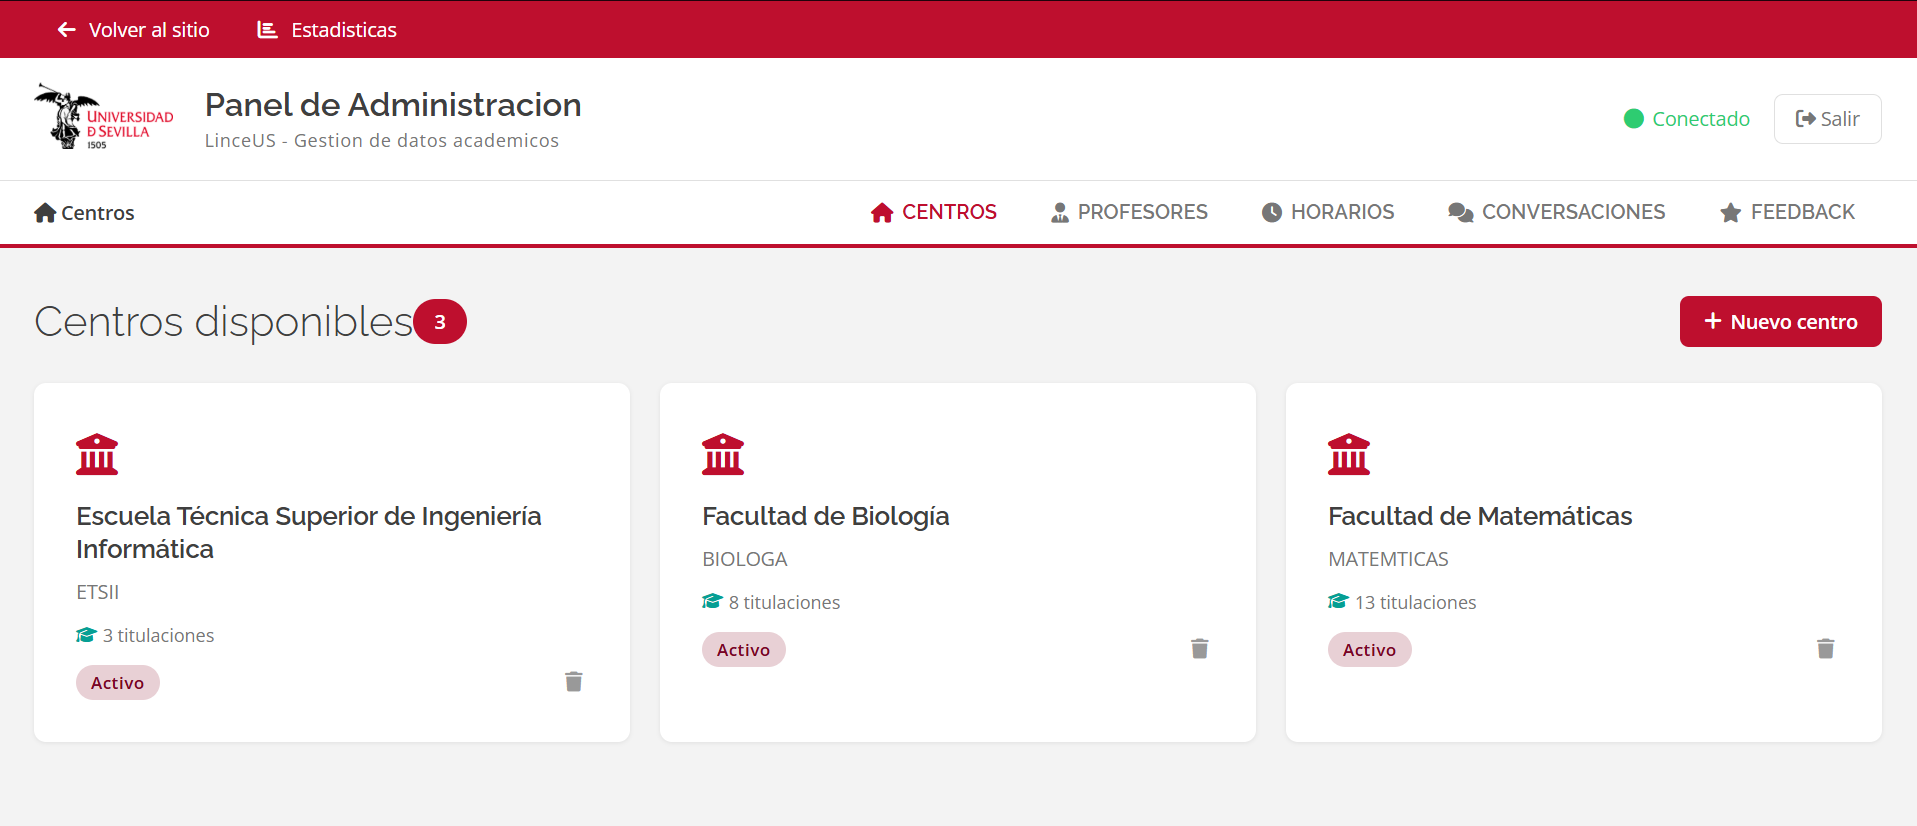
\includegraphics[width=0.95\linewidth]{img/admin_home.png}
\caption{Panel de administración: gestión de asignaturas.}\label{fig:admin-asignaturas}
\end{figure}

\begin{figure}[hbtp]
\centering
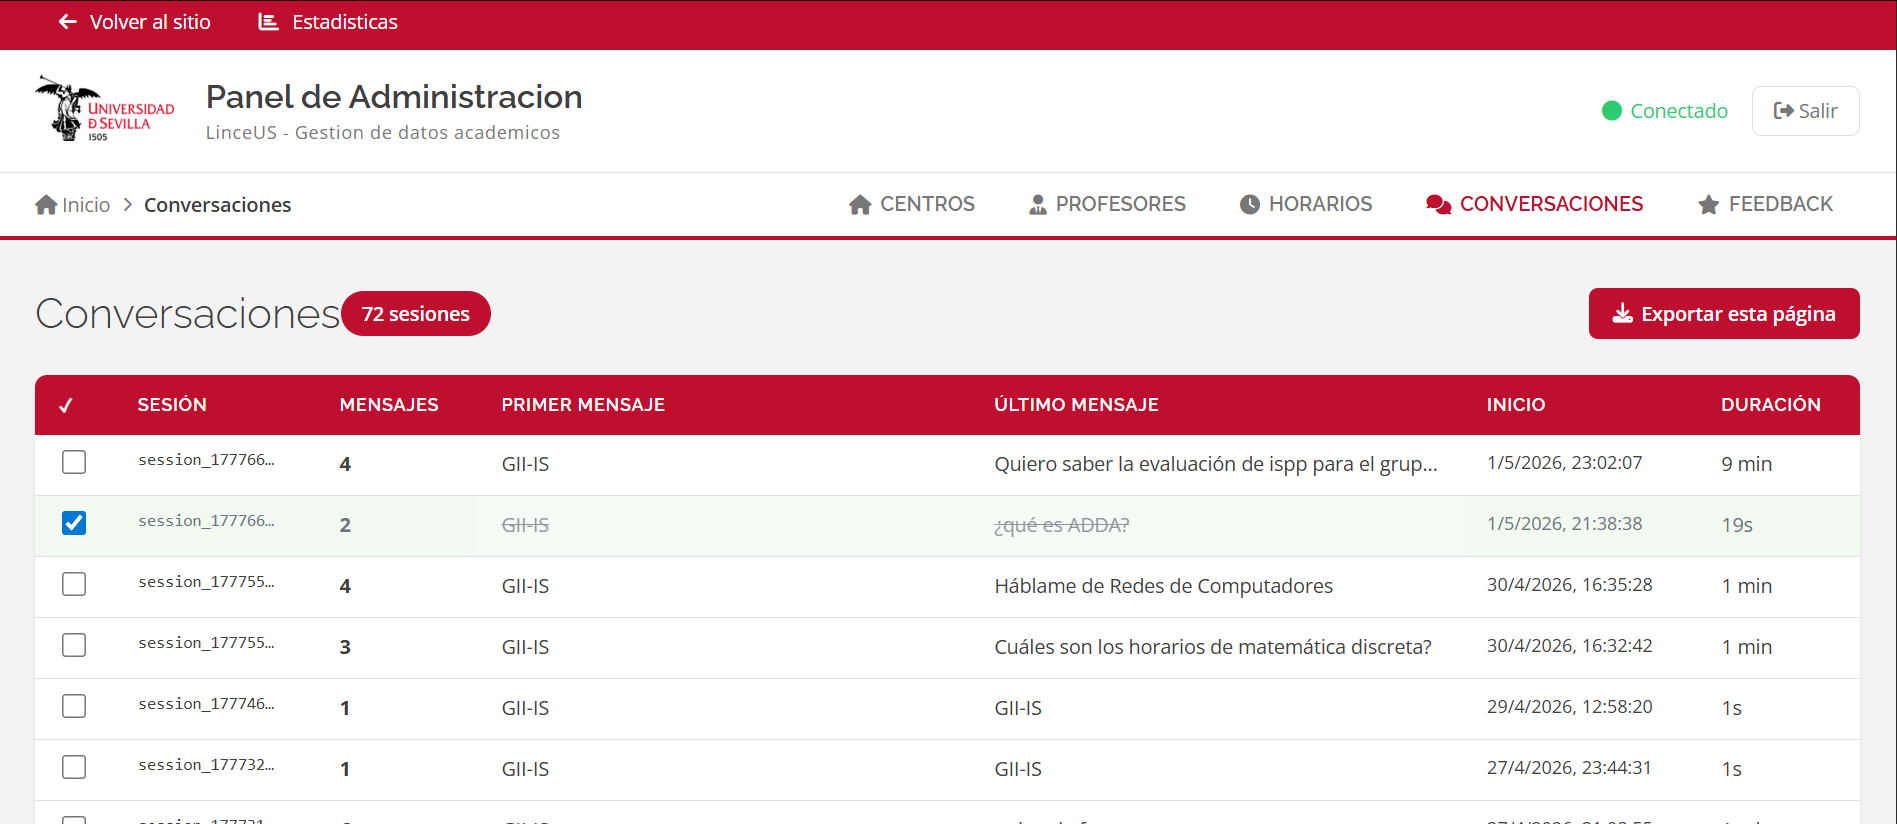
\includegraphics[width=0.95\linewidth]{img/admin_conversaciones.png}
\caption{Panel de administración: auditoría de conversaciones.}\label{fig:admin-conversaciones}
\end{figure}

\begin{figure}[hbtp]
\centering
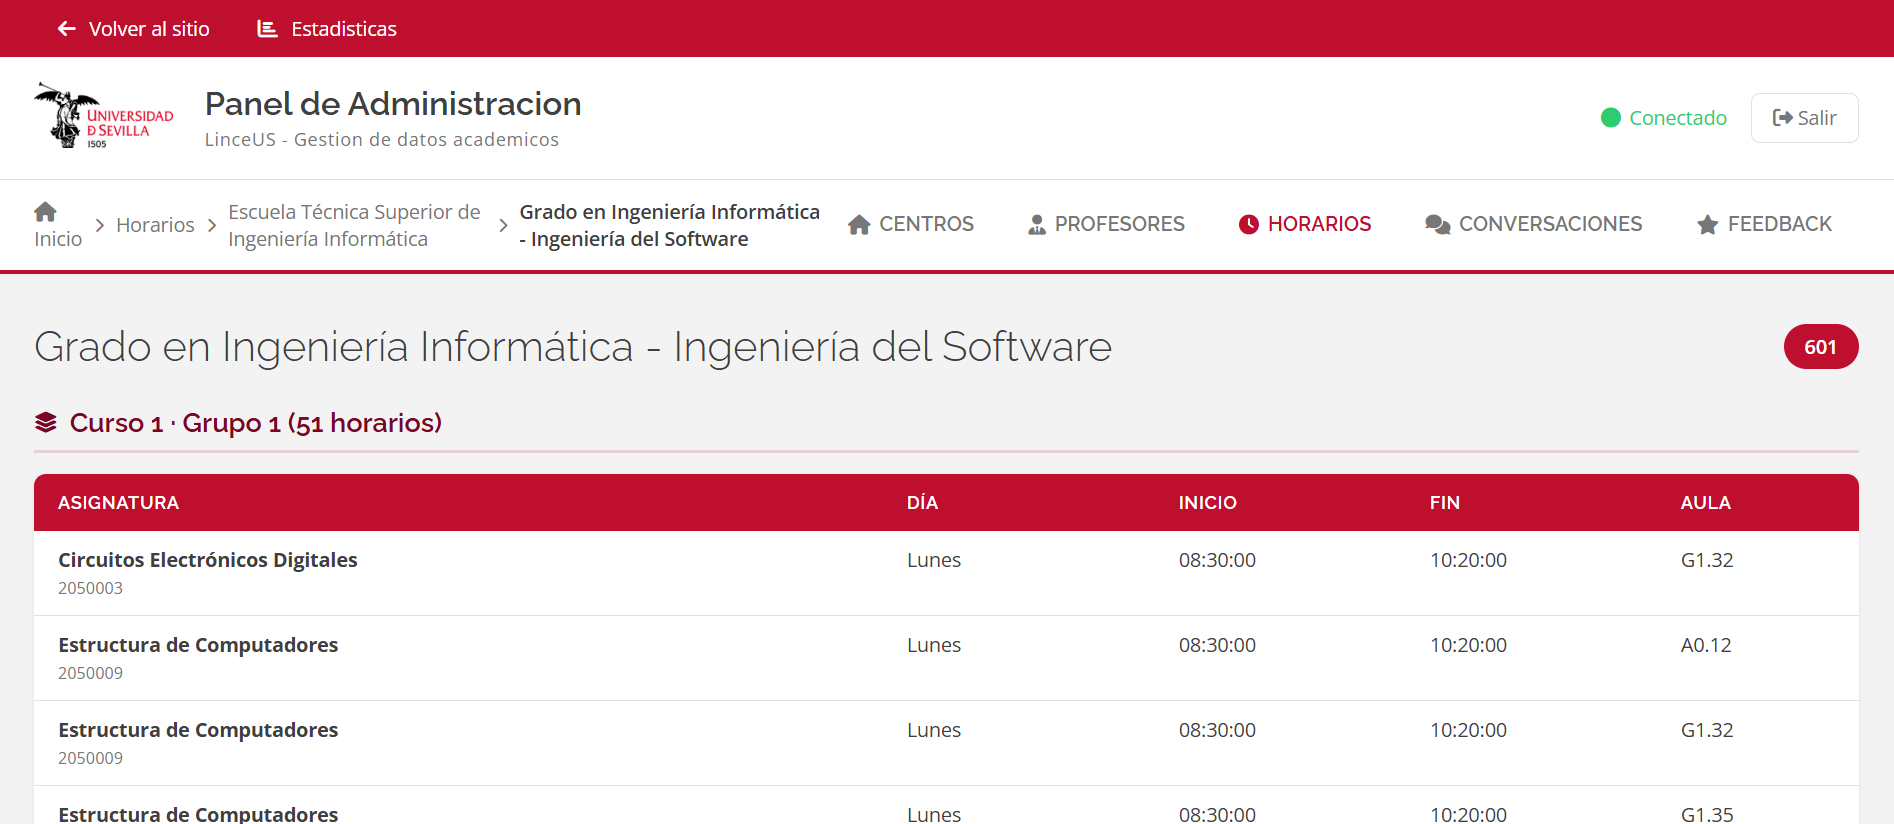
\includegraphics[width=0.95\linewidth]{img/admin_horarios.png}
\caption{Panel de administración: gestión de horarios.}\label{fig:admin-horarios}
\end{figure}

\begin{figure}[hbtp]
\centering
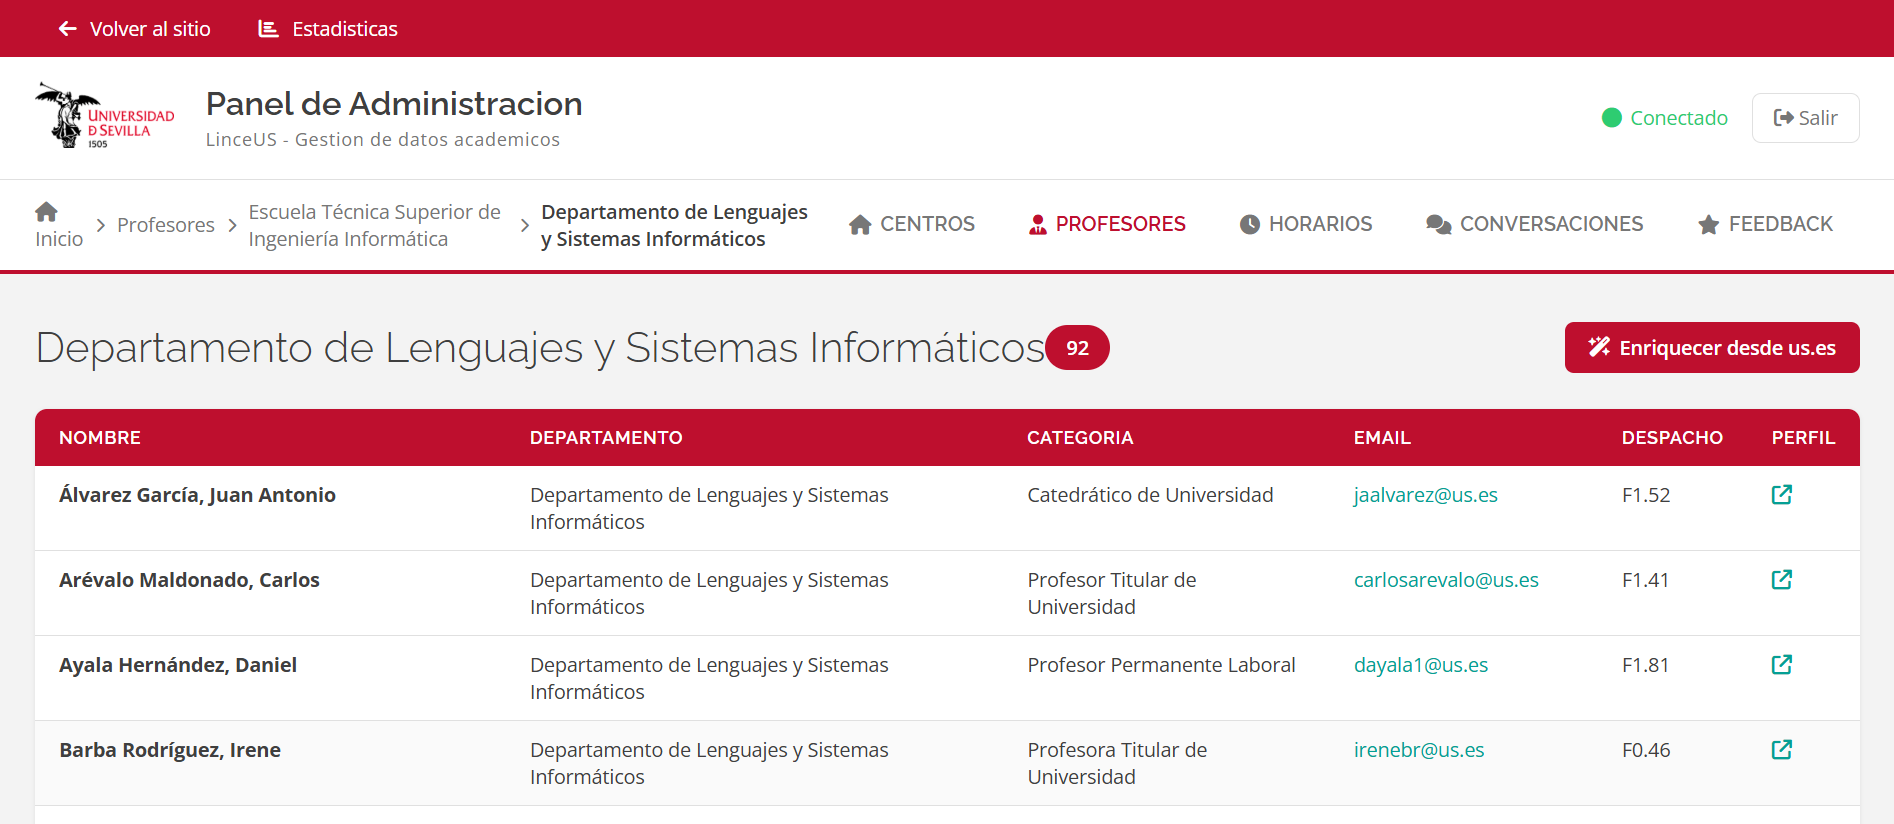
\includegraphics[width=0.95\linewidth]{img/admin_profesores.png}
\caption{Panel de administración: gestión de profesorado.}\label{fig:admin-profesorado}
\end{figure}

\section{Evolución del alcance respecto a la propuesta inicial}\label{sec:req-evolucion}

La propuesta original del proyecto, recogida en el anteproyecto~\cite{segura2024guiatfg}, contemplaba un alcance superior al efectivamente cubierto por el prototipo. La Tabla~\ref{tab:req-evolucion} resume las desviaciones principales y su justificación. En todos los casos las decisiones se han tomado con el objetivo de \textbf{garantizar la calidad de las funcionalidades implementadas}, antes que de cubrir un alcance amplio con calidad insuficiente, en línea con la recomendación de la guía de referencia.

\begin{table}[hbtp]
\centering
\small
\caption{Evolución del alcance respecto a la propuesta inicial.}\label{tab:req-evolucion}
\begin{tabular}{|p{3.0cm}|p{2.0cm}|p{7.5cm}|}
\hline
\textbf{Funcionalidad} & \textbf{Estado} & \textbf{Justificación} \\ \hline
\textit{Frontend} en React & Reformulado & Implementado en HTML/CSS/JavaScript \textit{vanilla} sobre \texttt{nginx}. La inversión de tiempo se ha priorizado en el desarrollo del chatbot, donde el valor añadido del proyecto es mayor. \\ \hline
Notificaciones \textit{push} a estudiantes & Aplazado & Sustituido por el \textbf{panel de administración}, que ofrece mayor valor a la persona que continúe el proyecto y materializa los requisitos de mantenibilidad y escalabilidad. \\ \hline
Soporte multilingüe (inglés) & Aplazado & El corpus académico es mayoritariamente español. Se aplaza a fase 2 cuando el sistema esté estabilizado y exista presupuesto para una segunda suite de pruebas. \\ \hline
Despliegue \textit{on-premise} & Reformulado & La información tratada es de carácter público y la sesión es anónima, por lo que no requiere despliegue en infraestructura propia. Se ha optado por DigitalOcean + Supabase. \\ \hline
Cambio dinámico de titulación & Añadido & Funcionalidad incorporada tras el feedback del piloto (D-029, D-030, D-053). No figuraba en la propuesta inicial. \\ \hline
Integración con \texttt{us.es} para profesorado & Añadido & Sustituye la propuesta inicial de \textit{scrapers} por departamento (D-043, D-044): fuente única, mantenible y completa. \\ \hline
Auditoría manual de conversaciones & Añadido & Surge como necesidad durante la fase de validación; permite la métrica de tráfico real post-despliegue (\S\ref{sec:pruebas-trafico}). \\ \hline
\end{tabular}
\end{table}

El balance final es satisfactorio: el sistema cubre con calidad los tres dominios académicos centrales de la propuesta y aporta dos funcionalidades no previstas (panel de administración y cambio dinámico de titulación) que refuerzan los requisitos de mantenibilidad y experiencia de usuario. Las funcionalidades aplazadas son recuperables en una segunda iteración sin necesidad de modificar el núcleo del sistema, lo que se discute con detalle en el Capítulo~\ref{cap:conclusiones}.
